%!TEX root = ProgCPP_ZF.tex

\part{Polymorphismus}
\textbf{Auftrag:} Stellen Sie bei allen Uhren die Zeit eine Stunde vor.
\begin{itemize}
	\item Obwohl der Auftrag völlig klar ist, hat man Mühe ihn auszuführen, weil jede Uhr auf eine andere Art verstellt wird.
	\item Der Auftrag ist recht abstrakt, die Ausführung ist aber sehr konkret, sobald sie wissen, welche Uhr sie verstellen müssen
\end{itemize}

\section{Static vs. Dynamic Binding}
\begin{itemize}
	\item Static Binding (early binding, statische Bindung)
	\begin{itemize}
		\item bereits zur Compilezeit wird festgelegt, welcher (Elementfunktions-) Code ausgeführt wird (Normalfall)
	\end{itemize}
	\item Dynamic Binding (late binding, dynamische Bindung)
	\begin{itemize}
		\item erst zur Laufzeit wird in Abhängigkeit des Objekts festgelegt, welcher (Elementfunktions-) Code ausgeführt wird
		\item Analogie: sobald sie wissen, welche Uhr sie verstellen müssen, können sie das konkrete Verfahren anwenden
		\item das ist das Konzept des Polymorphismus
	\end{itemize}
\end{itemize}

\subsection{Dynamic Binding}
\begin{itemize}
	\item ist der mächtigste OO-Mechanismus (oft präziser mit run-time polymorphism bezeichnet)
	\item Elementfunktionen, die dynamisch gebunden werden, muss bei der Deklaration das Schlüsselwort \textbf{virtual} vorangestellt werden (zwingend!)
	\begin{itemize}
		\item in der abgeleiteten Klasse soll (muss aber nicht) die Funktion auch mit virtual gekennzeichnet werden
	\end{itemize}
	\item Polymorphismus wird häufig als ineffizient bezeichnet, oft jedoch zu unrecht (mehr darüber im Vertiefungsmodul Embedded Software Engineering)
	\item Regeln:
	\begin{itemize}
		\item Eine Funktion soll dann als \textbf{virtual} deklariert werden, wenn sie in der abgeleiteten Klasse neu definiert (überschrieben) wird, sonst nicht! In diesem Fall muss auch der Destruktor \textbf{virtual} sein.
		\item Der Destruktor muss auch dann \textbf{virtual} sein, wenn ein Objekt einer Unterklasse dynamisch erzeugt wird und einem Pointer auf die Basisklasse zugewiesen wird (Substitutionsprinzip).
	\end{itemize}
	\item Achtung: nicht mit Funktionsüberladung (gleicher Name aber unterschiedliche Signatur) verwechseln!
\end{itemize}

\subsubsection{Beispiel: Zeichnen von geometrische Figuren}
\begin{itemize}
	\item Eine immer gleich heissende Elementfunktion draw() hat unterschiedliche Implementationen, je nach Art des aktuellen Objekts.
	\item Bsp.: Eine Zeichenfunktion für geometrische Objekte hat ganz unterschiedliche Implementationen, je nach dem ob es sich um einen Kreis, ein Rechteck, Textblock, Polygonzug, etc. handelt.
\end{itemize}

\subsection{Statischer vs. dynamischer Datentyp}
\noindent
\begin{minipage}{\linewidth}
	\begin{lstlisting}
	class Article;
	class Book : public Article {};
	Article* pa;
	pa = new Book;
	\end{lstlisting}
\end{minipage}
\begin{itemize}
	\item Der statische Datentyp bezeichnet den Datentyp bei der Deklaration $\rightarrow$ pa ist ein pointer auf Article
	\item Der dynamische Datentyp bezeichnet den effektiven Datentyp zur Laufzeit $\rightarrow$ pa ist ein Pointer auf Book
\end{itemize}

\subsection{Aufruf von virtuellen Elementfunktionen}
\begin{itemize}
	\item Virtuelle Elementfunktionen können sowohl dynamisch (über Pointer oder Referenzen) als auch statisch aufgerufen werden.
	\item Bei statischen Aufrufen erfolgt die Auswahl der richtigen Funktion bereits bei der Übersetzung (d.h. ohne Overhead)
	\begin{itemize}
		\item Dies ist dann der Fall, wenn das Objekt bereits zur Entwicklungszeit bekannt ist.
	\end{itemize}
	\item Bei dynamischen Aufrufen erfolgt die Auswahl der richtigen Funktion zur Laufzeit aufgrund des tatsächlichen (dynamischen) Typs des Objekts. Dies ist mit einem Overhead verbunden.
\end{itemize}

\subsubsection{Statischer Aufruf von virtuellen Elementfunktionen}
\noindent
\begin{minipage}{\linewidth}
	\begin{lstlisting}
	Duck donald;
	SuperHero luckyLuke;
	
	donald.print();		// Duck::print()
	luckyLuke.print();	// SuperHero::print()
	\end{lstlisting}
\end{minipage}

\subsubsection{Dynamischer Aufruf von virtuellen Elementfunktionen}
\noindent
\begin{minipage}{\linewidth}
	\begin{lstlisting}
	void printCC1(const ComicCharacter& c)
	{
		c.print();	// dynamische Aufloesung
	}
	
	void printCC2(const ComicCharacter* pc)
	{
		pc->print();	// dynamische Aufloesung
	}
	
	Duck donald;
	SuperHero luckyLuke;
	printCC1(donald);	// Duck::print()
	printCC2(&luckyLuke);	// SuperHero::print()
	\end{lstlisting}
\end{minipage}

\subsection{Polymorphe Klassen (Virtuelle Klassen)}
\begin{itemize}
	\item Eine Klasse, welche mindestens eine virtuelle Funktion deklariert, heisst virtuell (polymorph)
	\item Virtuelle Klassen bewirken einen Mehraufwand für den Compiler und sind darum langsamer in der Ausführung
	\item Funktionen sollten nur dann als virtuell deklariert werden, wenn sie in einer abgeleiteten Klasse überschrieben werden (sollen)
	\item Konstruktoren sind nie virtuell
	\item Destruktoren virtueller Klassen müssen immer als virtuell deklariert werden, sonst wird nur der Destruktor der Basisklasse aufgerufen
	\item Destruktoren müssen auch dann virtuell sein, wenn ein Heapobjekt über einen Pointer der Basisklasse freigegeben wird
	\item Nicht virtuelle Methoden dürfen nicht überschrieben werden	
\end{itemize}

\subsubsection{Repräsentation virtueller Objekte im Speicher}
\begin{minipage}{0.45\linewidth}
	\begin{itemize}
		\item In der Virtual Function Table (vtbl) vermerkt das System der Reihe nach die Adressen der für eine Klasse gültigen virtuellen Elementfunktionen
		\item Das System legt für jede polymorphe Klasse eine vtbl an
		\item Jedes Objekt einer polymorphen Klasse enthält einen Virtual Table Pointer (vptr), welcher auf die vtbl der entsprechenden Klasse zeigt
	\end{itemize}
\end{minipage}
\begin{minipage}{0.5\linewidth}
	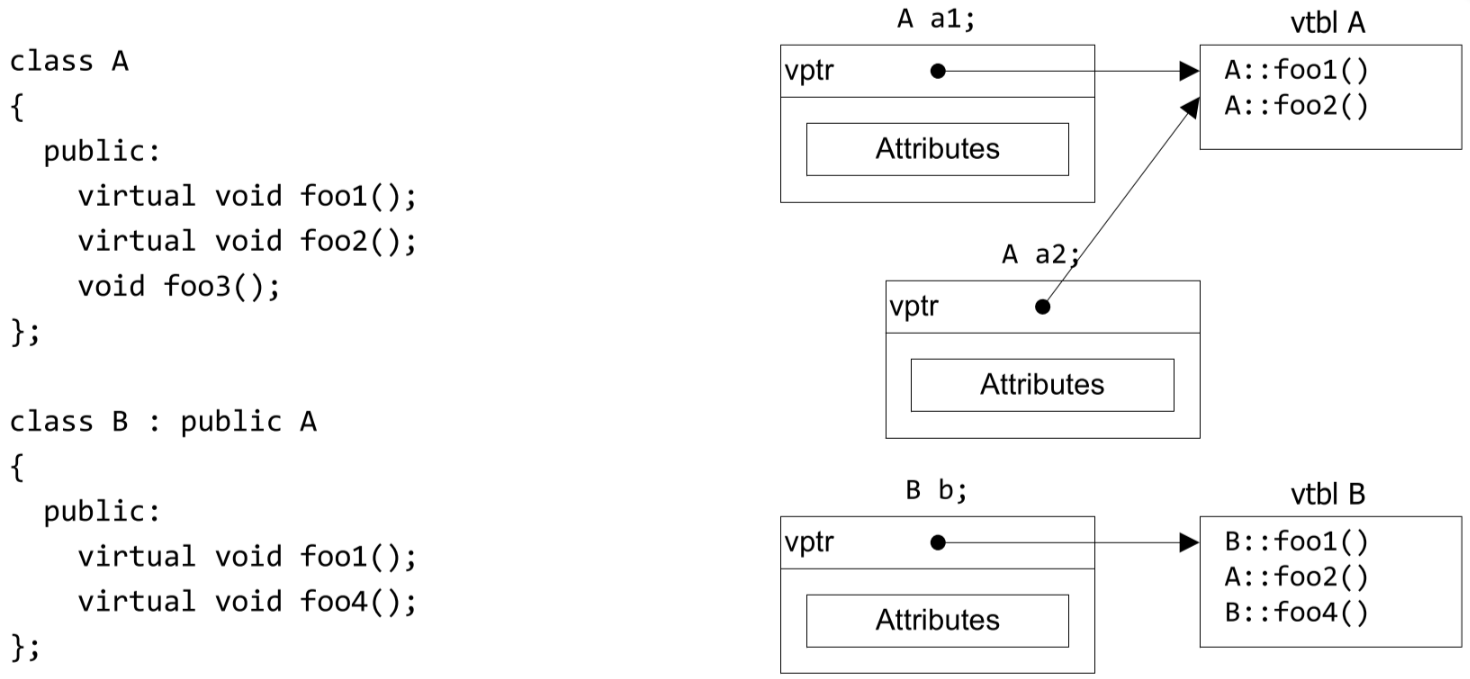
\includegraphics[width=\linewidth]{images/vtbl.png}
\end{minipage}

\section{Abstrakte Klassen}
\begin{itemize}
	\item Für manche Situationen sind die Vererbungsmechanismen, die wir bisher kennen gelernt haben, nicht ausreichend.
	\item Ein Kreis ist z.B. ein Spezialfall einer Ellipse. Es ist aber nicht sinnvoll, ihn so zu programmieren, da er sonst Eigenschaften erbt, die nicht verwendet werden.
	\item Es wäre möglich, Kreis und Ellipse als zwei unabhängige Klassen zu programmieren. Dann müssten aber alle Eigenschaften, die diese gemeinsam haben, doppelt programmiert werden.
	\item Dies versucht die objektorientierte Programmierung zu vermeiden.
	\item Es ist besser, die Eigenschaften, die Kreise und Ellipsen gemein haben, in einer Basisklasse zu programmieren.
	\item Die Kreis- und Ellipsenklassen erben dann parallel von der gemeinsamen Basisklasse.
	\item Die Basisklasse ist aber unvollständig, es handelt sich um eine abstrakte Klasse.
	\item Es können keine Objekte von abstrakten Klassen gebildet werden.
	\item In C++ können rein virtuelle Funktionen (pure virtual functions) deklariert werden, die in der Basisklasse nicht von einer Definition begleitet werden.
	\item Klassen, die mindestens eine rein virtuelle Funktion deklarieren, sind abstrakte Klassen
	\item Ist eine Klasse erst einmal als abstrakt definiert, kann diese nur durch Vererbung vervollständigt und dadurch nutzbar gemacht werden.
\end{itemize}

\subsection{Anwendungen von abstrakten Klassen (Beispiele)}
\begin{itemize}
	\item Definition von Schnittstellen (Interfaces)
	\begin{description}
		\item[Abstrakte Kommunikationsklasse] SerialCom, USB, Ethernet, etc. können davon sein
		\item[Abstrakte Printerklasse] Jeder Printertreiber erbt davon, bzw. implementiert dieses Interface. Die Hauptapplikation (z.B. Word) muss nicht geändert werden, wenn ein neuer Printertreiber implementiert wird.
	\end{description}
	\item "Real nicht existierende Abstrahierungen"
	\begin{itemize}
		\item ...von denen es keinen Sinn macht, ein Objekt zu erzeugen.
		\item Geometrische Figur als Gemeinsamkeit von Kreis, Rechteck, etc.
	\end{itemize}
\end{itemize}

\section{Mehrfachvererbung (Multiple Inheritance, MI)}
\begin{itemize}
	\item Manchmal ist es sinnvoll, eine abgeleitete Klassen von mehreren verschiedenen Basisklassen erben zu lassen.
	\item Wir sprechen dann von Mehrfachvererbung.
	\item Bei der Mehrfachvererbung werden die Basisklassen durch Komma getrennt:
	\subitem \textbf{class SingingWaiter : public Waiter, public Singer}
	\item Bei den Konstruktoren (Chaining) müssen die Konstruktoren der Basisklassen in der Ordnung gelistet werden, in der sie aufgerufen werden sollen.
\end{itemize}
\begin{multicols}{2}
	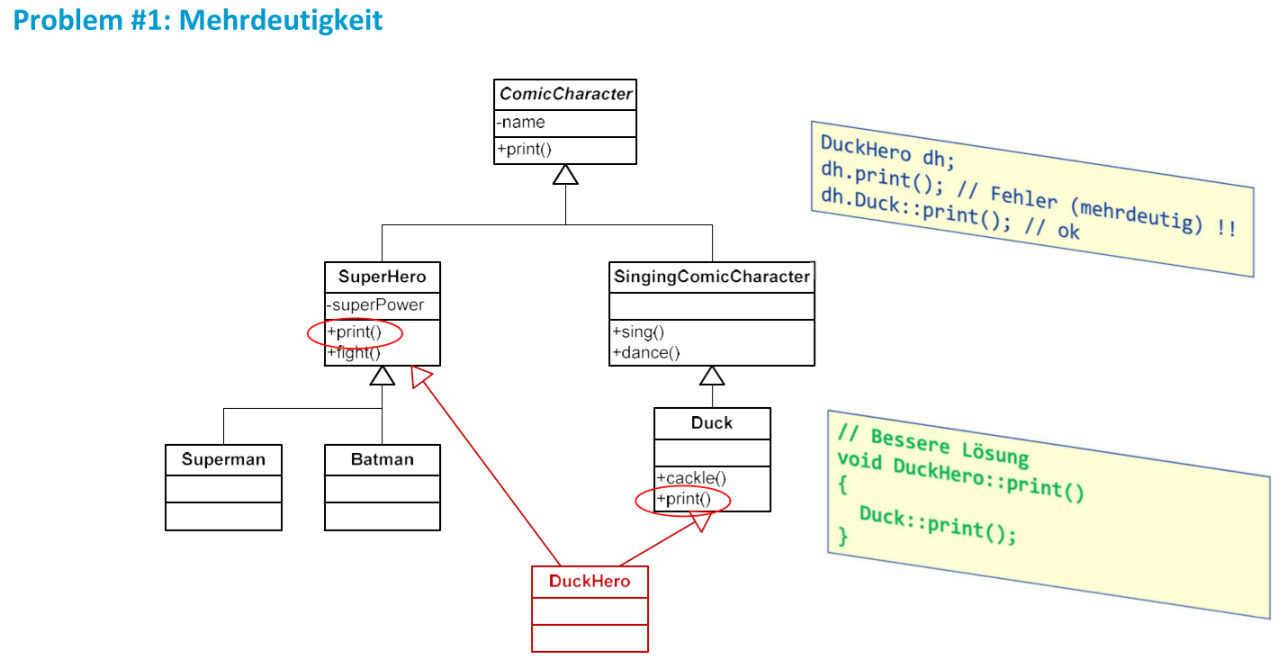
\includegraphics[width=\linewidth]{images/mehrdeutigkeit.png}
	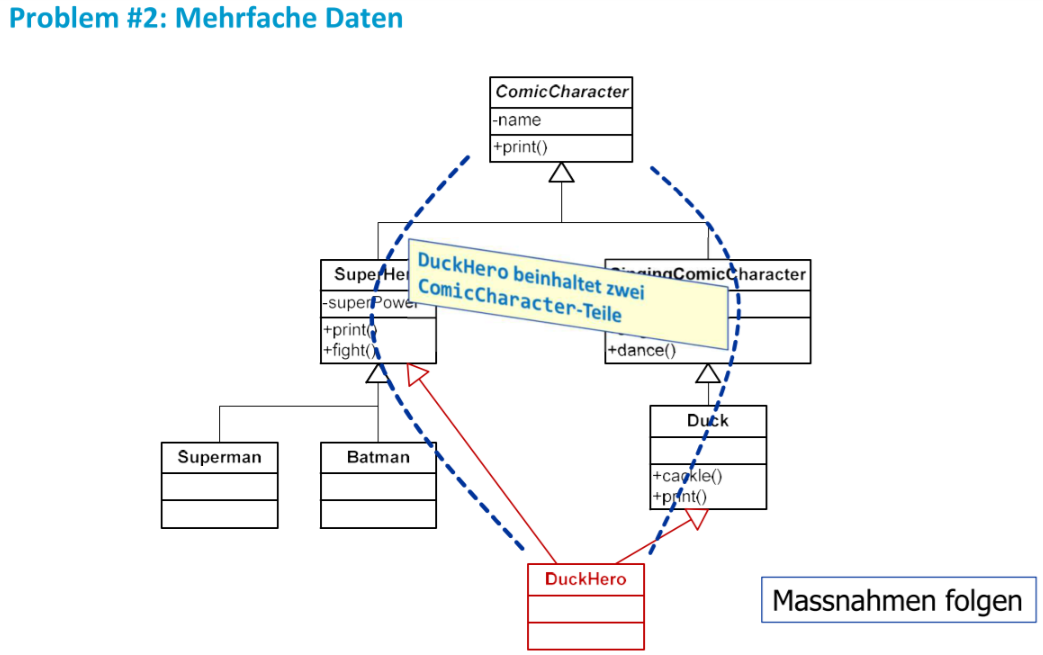
\includegraphics[width=\linewidth]{images/mehrfacheDaten.png}
\end{multicols}
\begin{itemize}
	\item Mehrfachvererbung ist ein sehr mächtiges Konzept, das (richtig eingesetzt) sehr nutzbringend sein kann. Bei schlechtem Einsatz der Mehrfachvererbung können enorme Probleme eingehandelt werden.
	\item Ein "guter" Einsatz der Mehrfachvererbung ist, wenn alle ausser höchstens einer Basisklasse ausschliesslich aus rein virtuellen Funktionen bestehen (Interfaces). Die neue Klasse implementiert dann die aufgelisteten Interfaces.
	\item Das ist die Art "Mehrfachvererbung", die auch in Java vorhanden ist: Vererbung gibt es nur einfach mit extends plus beliebige Implementationen von einem bis mehreren Interfaces mit implements
\end{itemize}

\subsection{Virtuelle Basisklassen}
Um zu vermeiden, dass bei Mehrfachvererbung eine gemeinsame Basisklasse mehrfach im Speicher vorkommt, kann virtuell geerbt werden.
\noindent
\begin{minipage}{\linewidth}
	\begin{lstlisting}
	class SingingComicCharacter : virtual public ComicCharacter
	{
		...
	};
	
	class SuperHero : virtual public ComicCharacter
	{
		...
	};
	\end{lstlisting}
\end{minipage}
In der Klasse DuckHero muss als erstes der ComicCharacter-Konstruktor aufgerufen werden.

\section{Laufzeit-Typinformationen (Run-Time Type Information, RTTI)}
\begin{itemize}
	\item Wie kann der (dynamische) Type eines polymorphen Objekts ermittelt werden?
	\item RTTI heisst der Mechanismus und \textbf{steht ausschliesslich für polymorphe Klassen zur Verfügung}
	\item Operator dynamic\_cast
	\item Operator typeid
	\item Struktur type\_info
\end{itemize}
\begin{achtung}
	RTTI sollte nur äusserst zurückhaltend eingesetzt werden!
\end{achtung}
\begin{itemize}
	\item Einsatz z.B. bei persistenten Objekten (um z.B. auch Klasseninformationen in einer rationalen Datenbank abzuspeichern)
\end{itemize}

\subsection{Operator dynamic\_cast}
\begin{itemize}
	\item Syntax: dynamic\_cast<SuperHero*>(p)
	\item Versucht, den Zeiger p in eine Zeiger auf ein Objekt des Typs SuperHero umzuwandeln.
	\item Der dynamische Datentyp von p ist massgebend.
	\item Umwandlung wird dann durchgeführt, wenn p tatsächlich auf ein Objekt vom Typ SuperHero, bzw. auf eine davon abgeleitete Klasse zeigt.
	\begin{itemize}
		\item Andernfalls ist das Resultat der Umwandlung der Nullpointer!
	\end{itemize}
\end{itemize}

\subsection{Operator typeid}
\begin{itemize}
	\item Ermitteln des dynamischen Datentyps eines polymorphen Objekts
	\item Ergibt eine Referenz auf ein Objekt des Typs type\_info. Diese Klasse beinhaltet u.a. eine Methode name(), welche den Namen der Klasse zurückgibt.
	\item Beispiel:
	\subitem cout << $"$p ist ein $"$ << typeid(*p).name() << $"$Objekt$"$;
\end{itemize}


